%Corps du document :
%\setlength{\parindent}{1cm}    

\section{Conception détaillée}

Attachons nous maintenant à la conception détaillée de notre application. Il s'agit
d'identifier et de spécifier les composants nécessaires pour automatiser tout ou
partie des outils à utiliser dans le cadre des cas d'utilisation identifiés.

Commençant par spécifier l'enchaînement des fenêtres grâce à un diagramme.

\subsection{Diagramme d'enchaînement des fenêtres}

\begin {center}
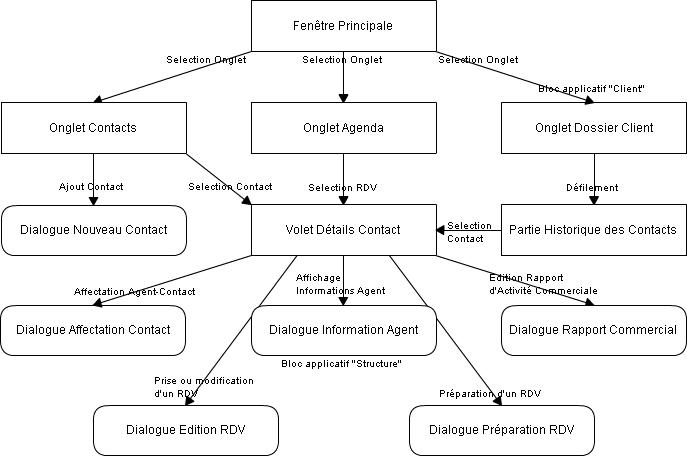
\includegraphics[width=\textwidth]{diagramme-edf.png}
\end {center}

\paragraph{Description}

L'Interface Homme-Machine (IHM) sera composée de trois onglets
principaux :

\begin{itemize}
\item \textbf{L'onglet Contacts} : Il présente la liste des Contacts prévus et affectés.
\item \textbf{L'onglet Agenda} : Il permet de consulter la liste des RDV pris.
\item \textbf{L'onglet Clients} : Cet onglet permet d'accéder aux dossiers des clients de la banque.
\end{itemize}

On observera également le volet \textbf{Détails du Contact}. Il permet d'effectuer toutes les
opérations nécessaires sur un Contact (une liste de ces services métiers se trouve plus loin
dans ce compte rendu).

\subsection{Dessin des fenêtres de l'IHM}

Voici une première représentation graphique de l'IHM que nous contruirons :

TODO @quentez

\subsection{Services Métiers invoqués par l'IHM}

Cette IHM utilise différents services métiers. En voici la liste :

\subsubsection{Services Métier Client}

\paragraph{Recherche de Clients}

\begin{itemize}
\item getAllClients()
\end{itemize}

\paragraph{Dossier Client}

\begin{itemize}
\item afficherInfos(idClient)
\item updateClient(client)
\end{itemize}

\subsubsection{Services Métier Agenda}

\begin{itemize}
\item getAgenda(type)
\item getSemaineParAgent(semaine,idAgent)
\item getJourAgence(date)
\item getPlageHoraire(idAgent,date)
\item planifierPlageAgenda(idAgent,typeActivite,date)
\item terminerPlanification()
\end{itemize}

\subsubsection{Services Métier Contact}

\paragraph{Recherche de Contacts}

\begin{itemize}
\item getAllContacts(idAgence)
\end{itemize}

\paragraph{Affectation des Contacts}

\begin{itemize}
\item getAllAgents(idAgence)
\item getContactsAgent(idAgent)
\item affecterContactAgent(idAgent,idContact)
\item transférerContact(idContact,idAgent)
\end{itemize}

\paragraph{Gestion d'un Contact}

\begin{itemize}
\item updateContact(contact)
\item annulerContact(idContact,raison)
\item changerEtatContact(date,idContact,etat)
\item confirmerContact(lettre)
\item réaliserContact(idContact)
\item regrouperContacts(liste<Contact>)
\item créerContactSpontané(date,idClient)
\end{itemize}

\paragraph{Préparation de l'entretien}

\begin{itemize}
\item consulterCatalogue(idSegment,idProduit)
\item préparerContact(idContact)
\item consulterPréparation(idContact)
\end{itemize}

\paragraph{Rapport d'activité commerciale}

\begin{itemize}
\item soumettreProposition(idContact,idOffre)
\item soumettreRapport{iContact,rapport}
\end{itemize}

\subsection{Spécification des Services Métier}

On ne détaillera que la liste des Services Métier invoqué par l'IHM dossier Client:

SM1: afficherInfo
\begin{itemize}
	\item SOM invoqués : SOMC1 : Consultation informations client
	\item Entrées : idClient
	\item Sorties : NomClient, Adresse, Comptes,....
	\item Procédure :
	\begin{itemize}
		\item Rechercher les informations le client (personne,compte): SOMC5.
	\end{itemize}
\end{itemize}

SM2 : updateClient
\begin{itemize}
	\item SOM invoqués : SOMC2 : Mise à jour des informations client
	\item Entrées : NomClient/Adresse/Compte/... (uniquement ceux modifiées)
	\item Sorties : null
	\item Procédure :
	\begin{itemize}
		\item Mettre à jour les informations sur le client (personne,compte): SOMC4.
	\end{itemize}
\end{itemize}

\subsection{Spécification des Services Objets Métier}

On ne détaillera que les Services Objets Métier concernant le bloc Client:


OM Client SOMC1 : getInfo
\begin{itemize}
\item Entrées : idClient
\item Sorties : NomClient, Adresse, Comptes,...
\item Entités/Classes : Client, Personne, Adresse, Compte
\item Permet de consulter toutes les informations d'un client.
\end{itemize}

OM Client SOMC2 : updateInfo
\begin{itemize}
\item Entrées : idClient, info
\item Sorties : null
\item Entités/Classes : Client, Personne, Adresse, Compte
\item Permet de mettre à jour des informations sur un client.
\end{itemize}

OM Client SOMC3 : getAll
\begin{itemize}
\item Entrées : null
\item Sorties : liste Client: NomClient, Adresse,...
\item Entités/Classes : Client, Personne, Adresse, Compte
\item Permet de consulter la liste de tous les clients.
\end{itemize}

\subsection{Spécification des IHM}
La connexion se faire de manière authentifier, en choisissant son rôle et en indiquant le mot de passe correspondant.
\includegraphics[width=\textwidth]{../../ihm/pngIHM/login.png}

L'onglet \textit{Contacts } permet d'afficher par défaut tous les contacts de l'agent actuellement connecté, avec la possibilité d'afficher également les contacts d'un autre agent si besoin. Le panneau de droite présente de manière concise les informations sur ce contact, avec la possibilité d'accéder aux informations clients en un clic.
Comme on l'a vu lors de la revue, le sélecteur d'état sur le contact ne sera utilisé que comme un filtre et non comme un moyen de changer l'état d'un contact. Le changement d'état se fera de manière automatique avec les actions correspondantes.
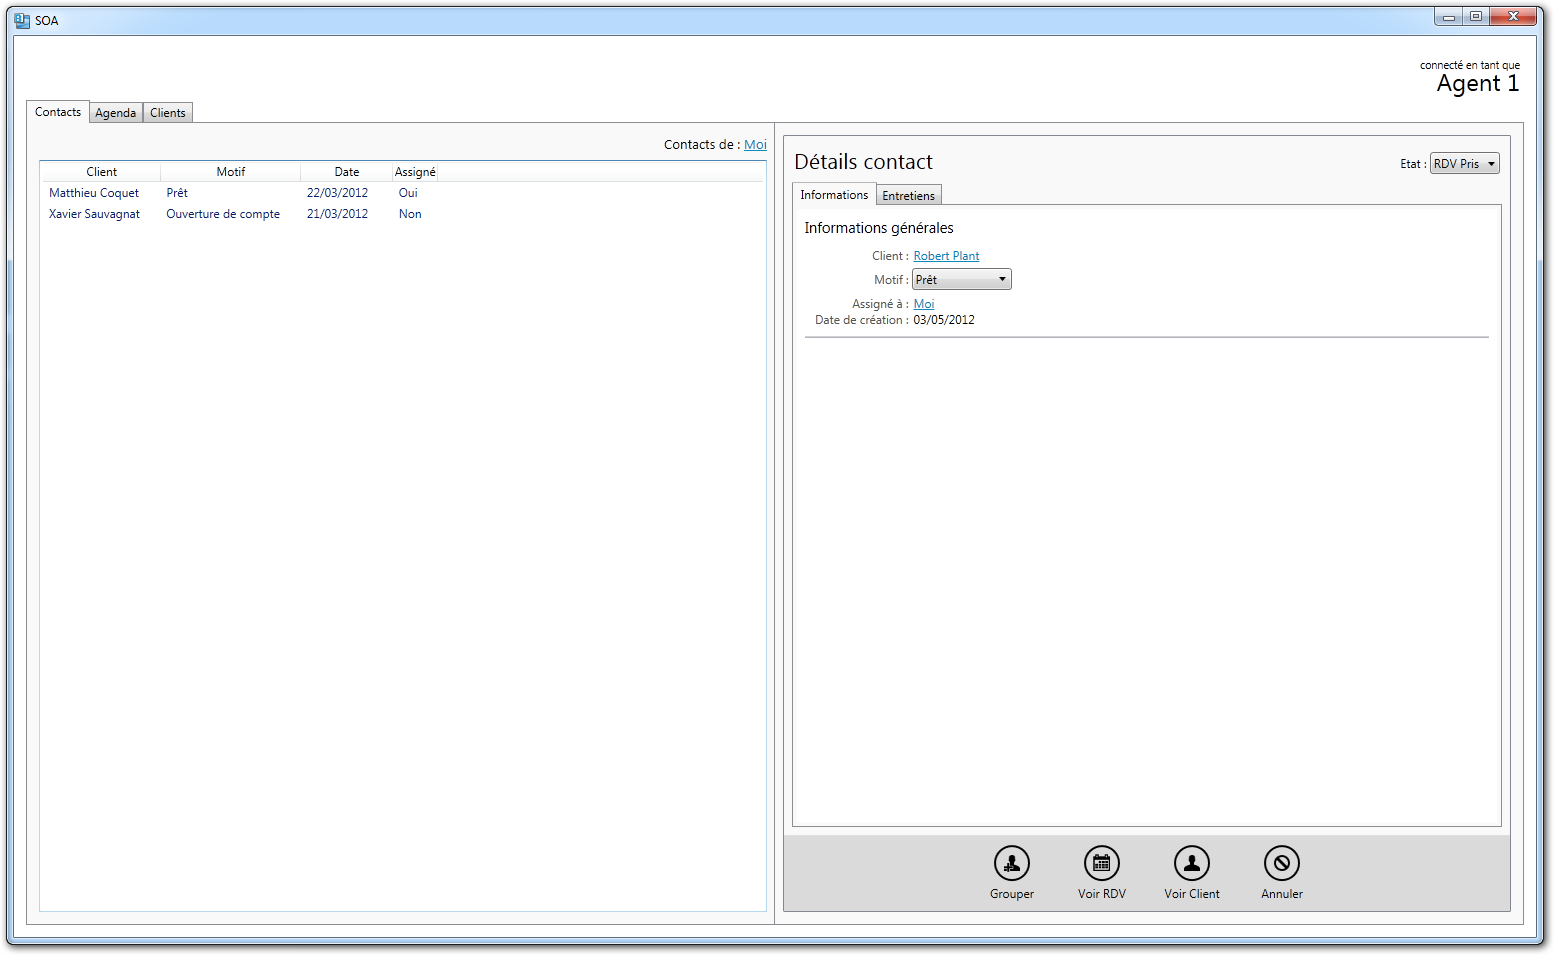
\includegraphics[width=\textwidth]{../../ihm/pngIHM/ListeContacts.png}

Dans la partie gauche, l'onglet \textit{Entretiens} permet visualiser sur un calendrier la date du rendez-vous et également de préparer l'entretien. C'est le même affichage pour la préparation que lors de l'entretien.
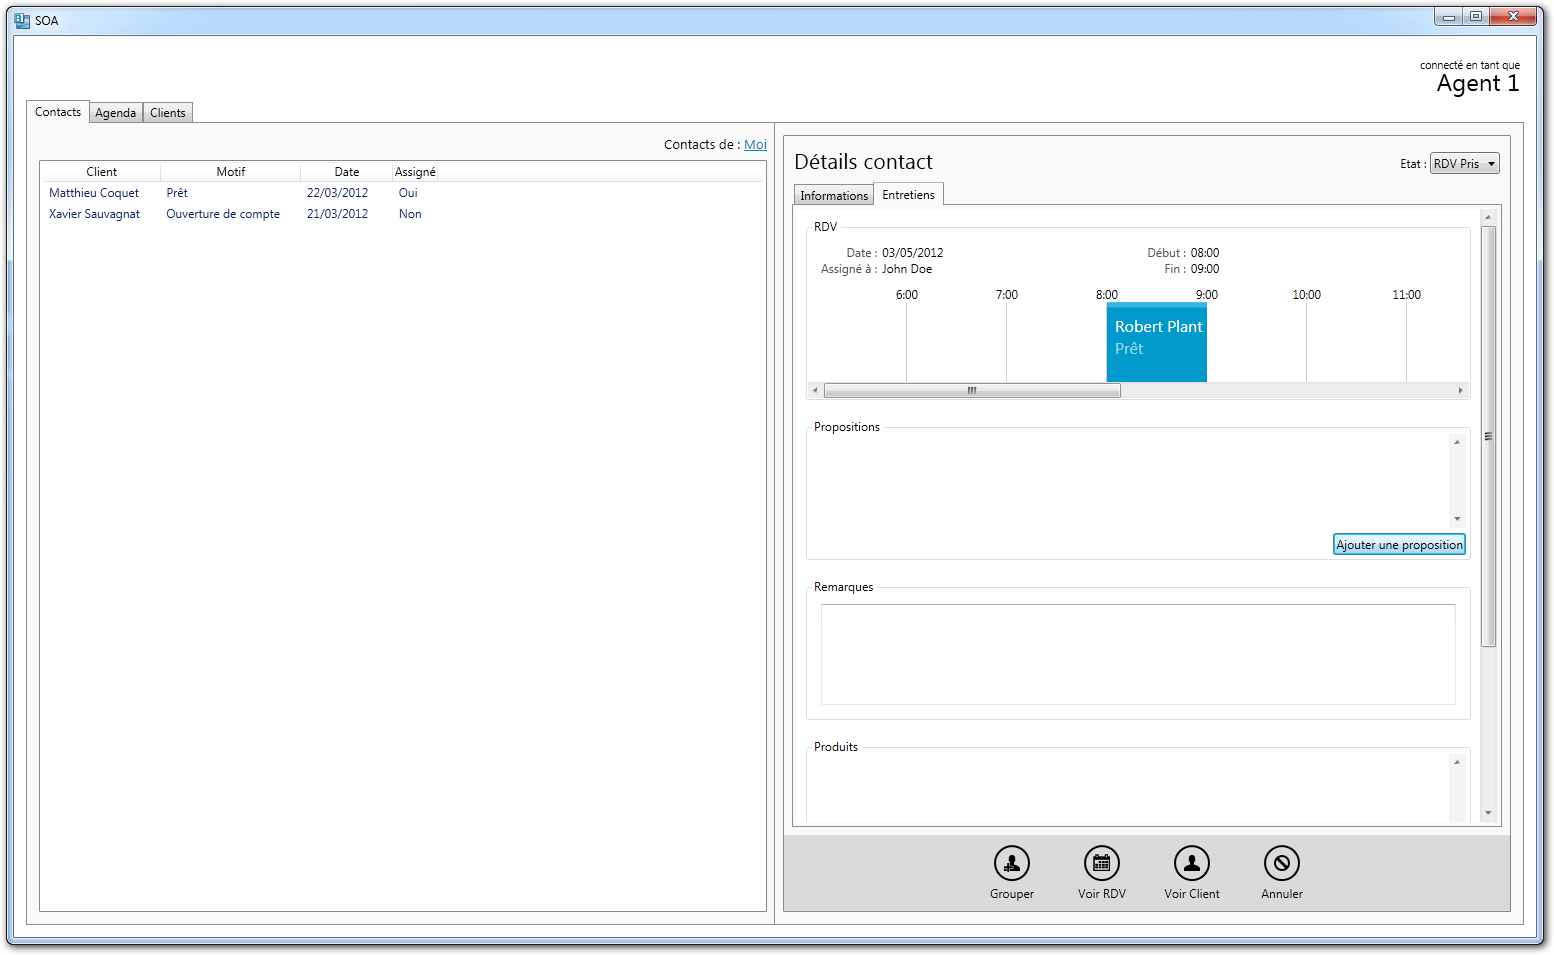
\includegraphics[width=\textwidth]{../../ihm/pngIHM/ContactEntretiens1.png}

Toujours dans l'onglet \textif{Entretiens}, en scrollant vers le bas, on dispose des champs nécessaires pour marquer les produits auxquel le contact à souscrit lors de l'entretien ainsi que pour rédiger le rapport qui clotûre l'entretien.
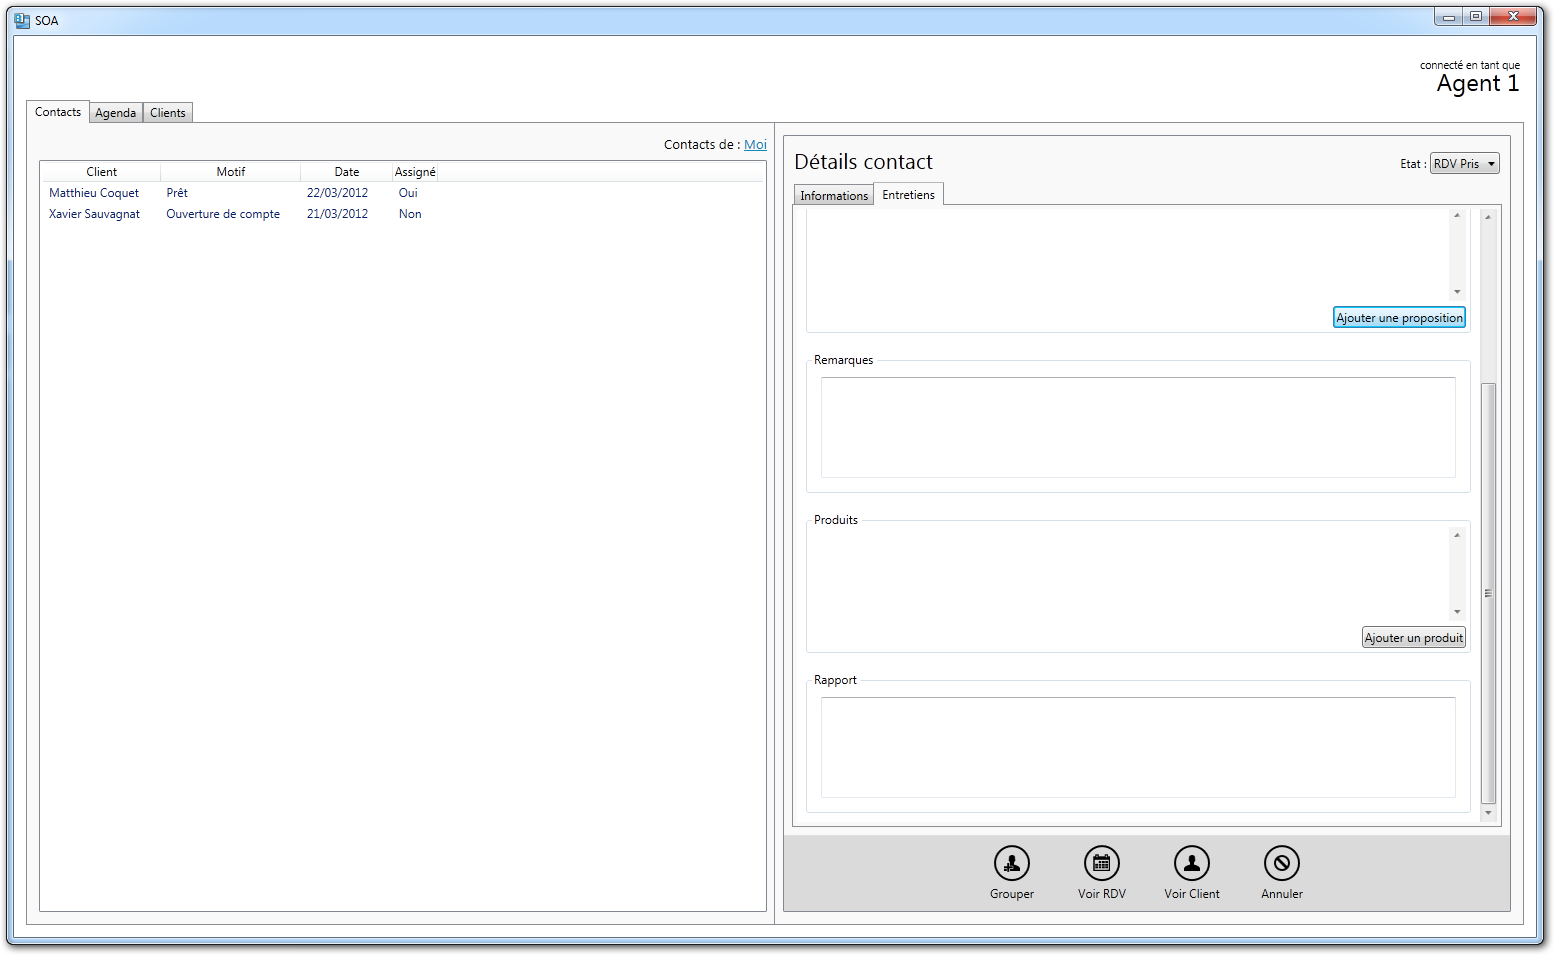
\includegraphics[width=\textwidth]{../../ihm/pngIHM/ContactEntretiens2.png}

Il s'agit de la fenêtre qui s'ouvre lorsqu'on souhaite afficher des contacts qui n'appartiennent pas à l'agent connecté, il s'agit simplement de sélectionner l'agent pour lequel on souhaite voir ces contacts.
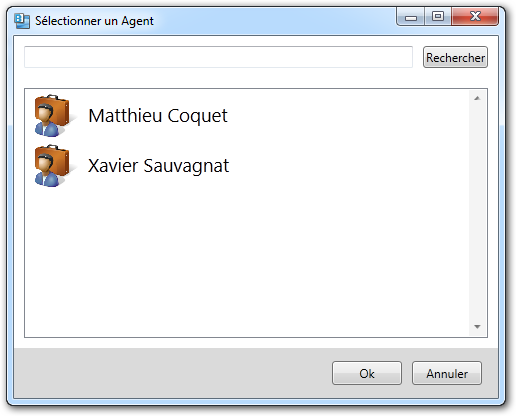
\includegraphics[width=\textwidth]{../../ihm\pngIHM/ChoixAgent.png}

L'onglet \textit{Agenda} offre 2 types de visualisation, ici nous avons la vue hebdomadaire, qui permet de voir sur la partie gauche le calendrier et sur la partie droite les informations sur la plage horaire selectionnée.
On notera la présence d'un bouton permettant de réaliser un contact spontanée.
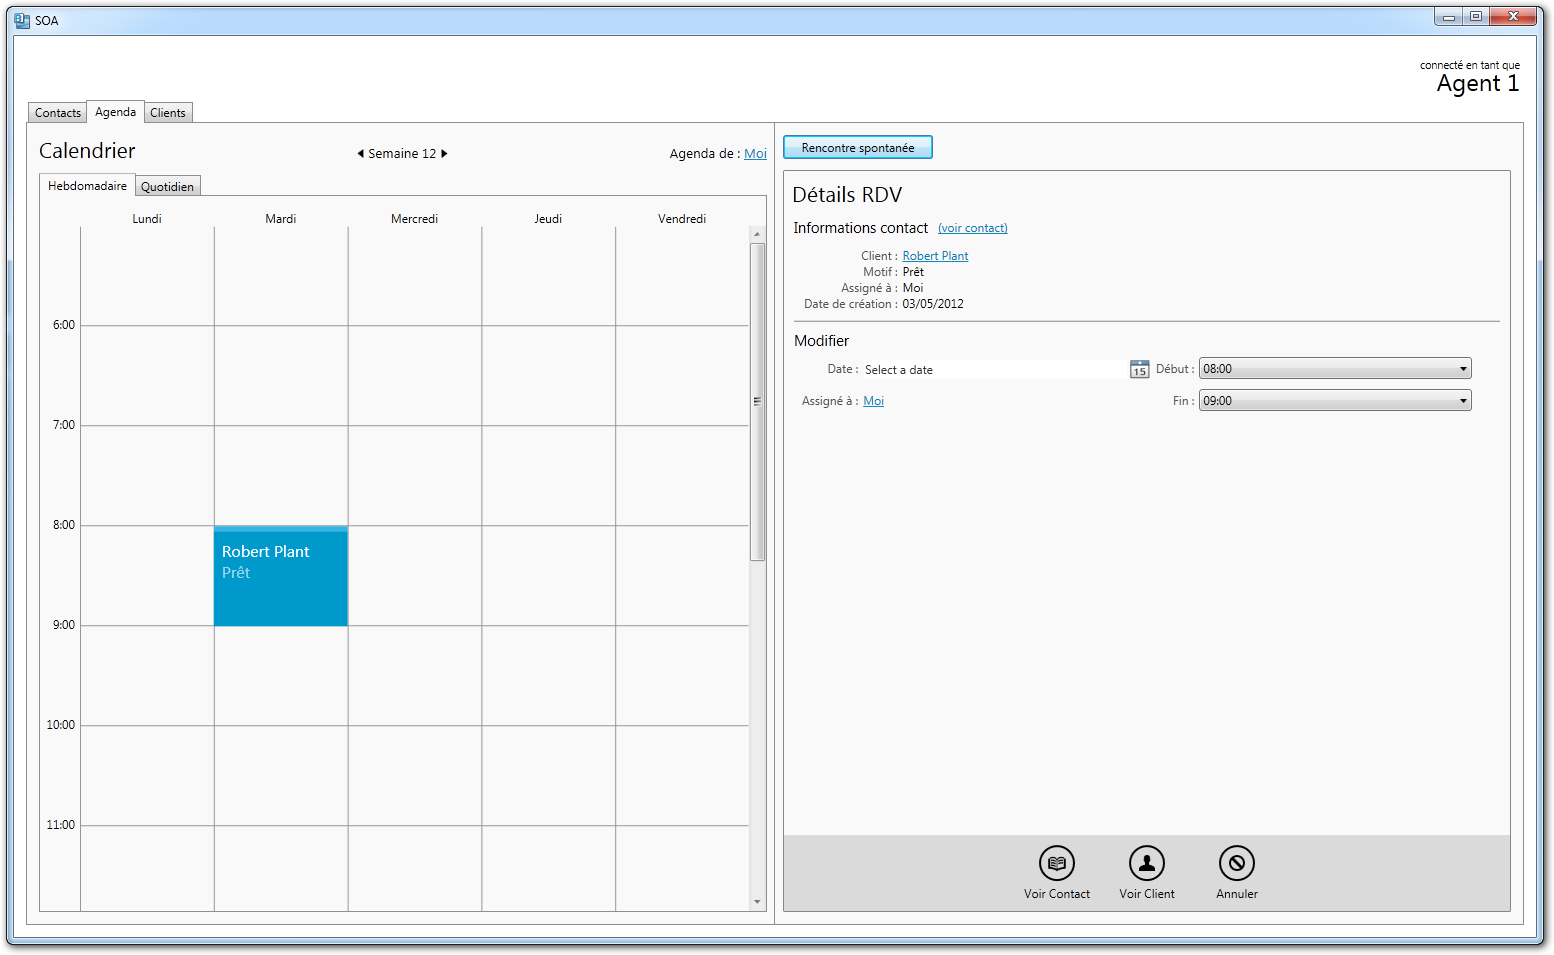
\includegraphics[width=\textwidth]{../../ihm/pngIHM/Calendrier Hebdomadaire.png}

La vue de l'agenda quotidenne se présente sous la même forme que la vue hebdomaire, sauf du point de vue du calendrier bien entendu.
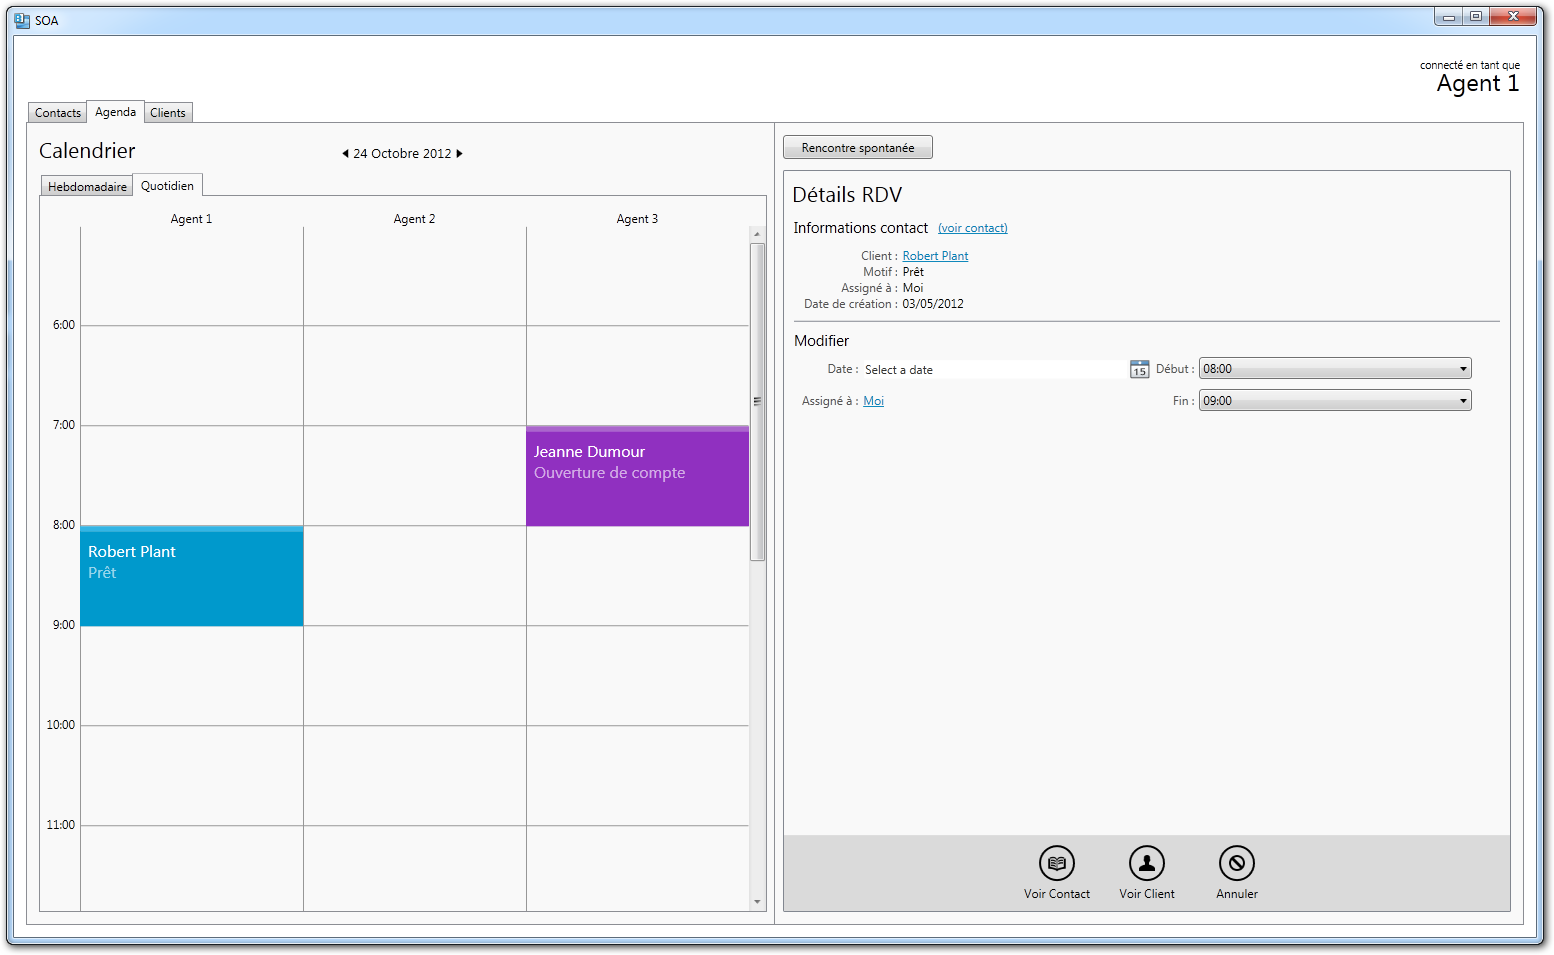
\includegraphics[width=\textwidth]{../../ihm/pngIHM/CalendrierQuotidien.png}

L'onglet \textit{Clients} permet de visualiser la liste des clients à gauche et de voir toutes les informations sur le client selectionné à droite, avec 3 onglets suivant les données que l'on souhaite consulter.
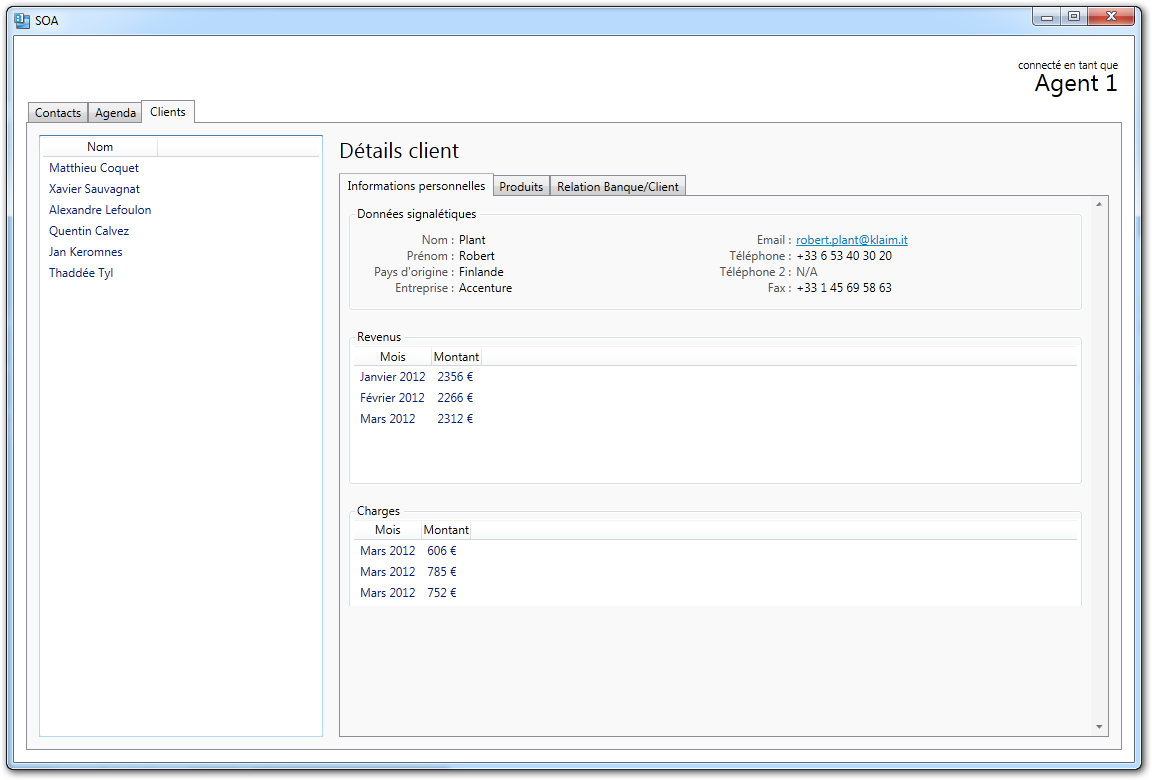
\includegraphics[width=\textwidth]{../../ihm/pngIHM/ListeClients.png}

Cette fenêtre permet de répondre au cas d'utilisation 6, où un agent obtient un entretien de manière spontanée, elle permet donc de renseigner le nom du client, la date et le motif ainsi que le type d'activité.
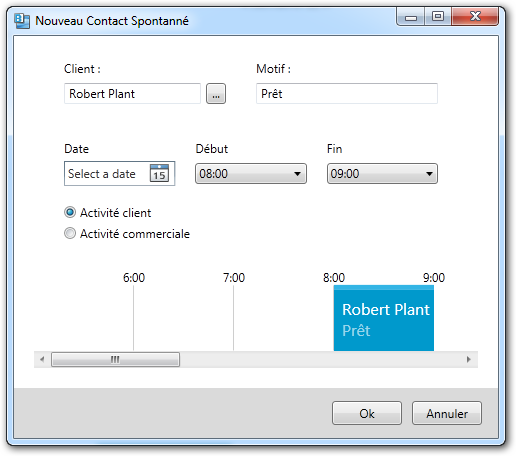
\includegraphics[width=\textwidth]{../../ihm/pngIHM/NouveauContactSpontanne.png}


